\documentclass[exercice,a4]{thedocument}%
\usepackage{texmaths-tikz}%
\usepackage[np]{numprint}%
\startdatakeys
\source{24GENMATAN1}
\BO{2026}
\cycle{4}
\competencesDuSocle{CA,CO}
\objectifsApprentissage{C4D1aa,C4D2aa,C4D3ac,C4D3ba,C4D3bb}
\motsCles{fonction linéaire,fonction affine,proportionnalité,graphique}
\enddatakeys
\begin{document}%
Un cinéma propose trois tarifs :

\textbf{Tarif « Classique » :} la personne paye chaque entrée 11~\euro.

\textbf{Tarif « Essentiel » :} la personne paye un abonnement annuel de
50~\euro{} puis chaque entrée coûte 5~\euro.

\textbf{Tarif « Liberté » :} la personne paye un abonnement annuel de
240~\euro{} avec un nombre d'entrées illimité.

\begin{enumerate}
    \item Avec le tarif « Classique », une personne souhaite acheter trois
    entrées au cinéma. Combien va-t-elle payer ?
    \item Avec le tarif « Essentiel », une personne souhaite aller huit fois
    au cinéma. Montrer qu'elle va payer 90~\euro.
    \item Dans la suite, $x$ désigne le nombre d'entrées au cinéma.
    On considère les trois fonctions suivantes :
    \[
        f:x\longmapsto 50+5x,\qquad
        g:x\longmapsto 240,\qquad
        h:x\longmapsto 11x.
    \]
    Associer, sans justifier, chacune de ces fonctions au tarif correspondant.
\end{enumerate}

Le graphique ci-dessous représente le prix à payer en fonction du nombre
d'entrées pour chacun de ces trois tarifs.

\begin{center}
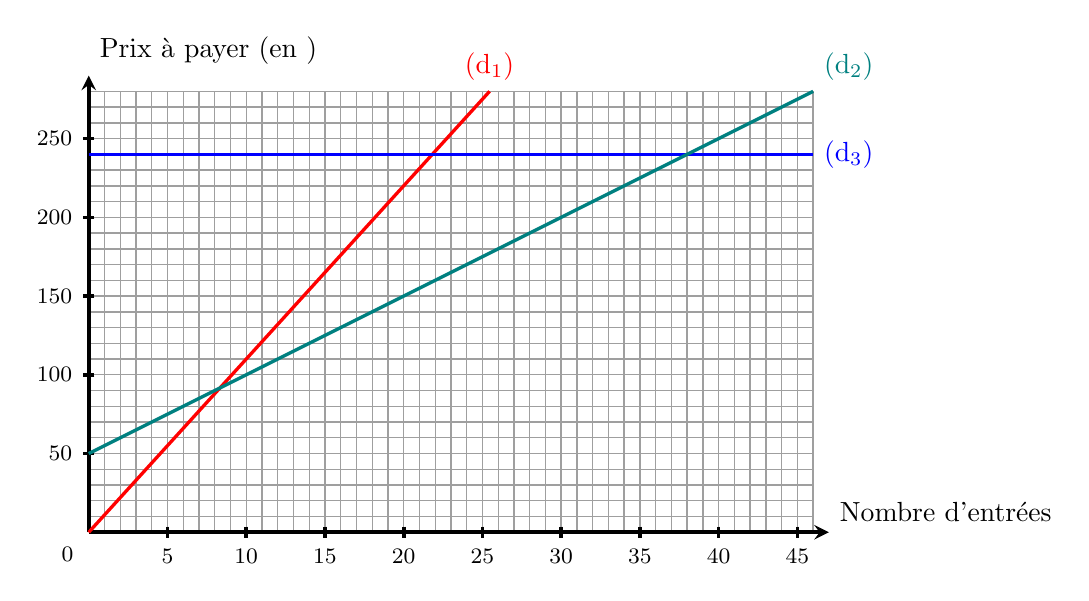
\begin{tikzpicture}[x=2mm,y=0.2mm,>=stealth]
    \draw[color=gray!75,line width=0.5pt,xstep=1,ystep=10] (0,0) grid (46,280);
    \draw[->,line width=1.3pt] (0,0)--(47,0) node[above right]{Nombre d'entrées};
    \foreach \x in {5,10,...,45}
        \draw[shift={(\x,0)},line width=1.3pt]
            (0pt,2pt)--(0pt,-2pt) node[below,fill=white]{\footnotesize $\np{\x}$};
    \draw[->,line width=1.3pt] (0,0)--(0,290)
        node[above right]{Prix à payer (en \euro{})};
    \foreach \y in {50,100,...,250}
        \draw[shift={(0,\y)},line width=1.3pt]
            (2pt,0pt)--(-2pt,0pt) node[left,fill=white]{\footnotesize $\np{\y}$};
    \draw[color=black] (-2pt,-2pt) node[below left]{\footnotesize 0};
    \draw[line width=1.2pt,color=red] (0,0)--(25.4545,280)
        node[above]{$(\mathrm{d}_1)$};
    \draw[line width=1.2pt,color=blue] (0,240)--(46,240)
        node[right]{$(\mathrm{d}_3)$};
    \draw[line width=1.2pt,color=teal] (0,50)--(46,280)
        node[above right]{$(\mathrm{d}_2)$};
\end{tikzpicture}
\end{center}

La droite $(\mathrm{d}_1)$ représente la fonction correspondant au tarif
« Classique ». La droite $(\mathrm{d}_2)$ représente la fonction
correspondant au tarif « Essentiel ». La droite $(\mathrm{d}_3)$ représente
la fonction correspondant au tarif « Liberté ».

\begin{enumerate}
    \setcounter{enumi}{3}
    \item Quel tarif propose un prix proportionnel au nombre d'entrées ?
    \item Pour les questions suivantes, aucune justification n'est attendue.
    \begin{enumerate}
        \item Avec 150~\euro, combien peut-on acheter d'entrées au maximum
        avec le tarif « Essentiel » ?
        \item À partir de combien d'entrées le tarif « Liberté » devient-il
        le tarif le plus intéressant ?
        \item Si on décide de ne pas dépasser un budget de 200~\euro, quel
        est le tarif qui permet d'acheter le plus grand nombre d'entrées ?
    \end{enumerate}
\end{enumerate}
\showthesource
\end{document}
